
\noindent 
\textbf{\stepcounter{zadatak}
\thecjelina.\thezadatak.}
Koeficijent kinetičkog trena između blokova i podloge je $\mu_k=0,2$, a dimenzije i mase su: $a=5\ m$, $b=3\ m$, $v=4\ m$, $m_A=10\ kg$ i $m_B=15\ kg$.
Koliki je iznos ubrzanja blokova prikazanih na slici?
\begin{figure}[ht]%{r}{0.7\textwidth} % Inline image example
  \begin{center}
    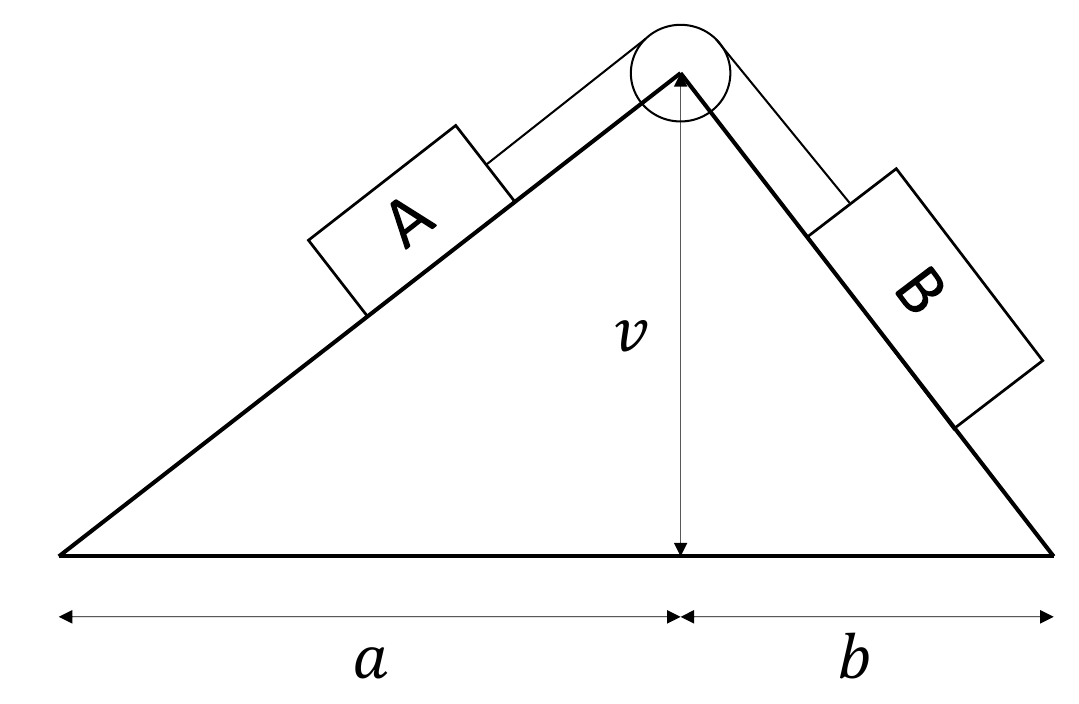
\includegraphics[scale=0.20]{../03_Dinamika_materijalne_tocke/Zadatak_D705.png}
  \end{center}
  %\caption{Fish}
\end{figure}

